\chapter{\textit{tanksEnv}}

This chapter presents \textit{tanksEnv}, a tanks battle ground environment. It is based on the environment developed in \cite{boeckx}.\textit{tanksEnv} is a grid-like environment of finite size. Two teams are playing against each other: team "red" and team "blue". 

\section{Tanks} 

Each team is composed of one or several players (let's call them tanks) that are defined by their states, which contain the same information for each tank, that is:

\begin{itemize}
    \item The position of the tank in (x,y) coordinates
    \item An id that is different from all tanks (of both teams)
    \item Its team
    \item How much ammo it has left
    \item Which other tank it's aiming at
    \item Whether it is still in the game or has been hit and can no longer move or shoot
\end{itemize}

\section{Actions}

The different available actions are:

\begin{itemize}
    \item \textit{nothing}: Do nothing.
    \item \textit{north}, \textit{south}, \textit{east}, \textit{west}: Move in one of the cardinal directions, if there is nothing preventing the tank from doing so (obstacle, other tank, edge of the grid).
    \item \textit{aim-i}: Aim at tank i (tank which id is i), if this tank is visible by the tank that tries to execute the action.
    \item \textit{shoot}: Shoot at the tank previously aimed at, if it is visible and action \textit{aim-i} has already been carried out.
\end{itemize}
\hfill\break

When taking action \textit{shoot}, there is a certain probability to kill the target, that depends on the range to the target. This is shown on figure \ref{fig:Pkill}. Explanations about how it was determined are to be found in appendix \ref{ann:pkill}.

\begin{figure}[h!] \label{fig:Pkill}
    \centering
    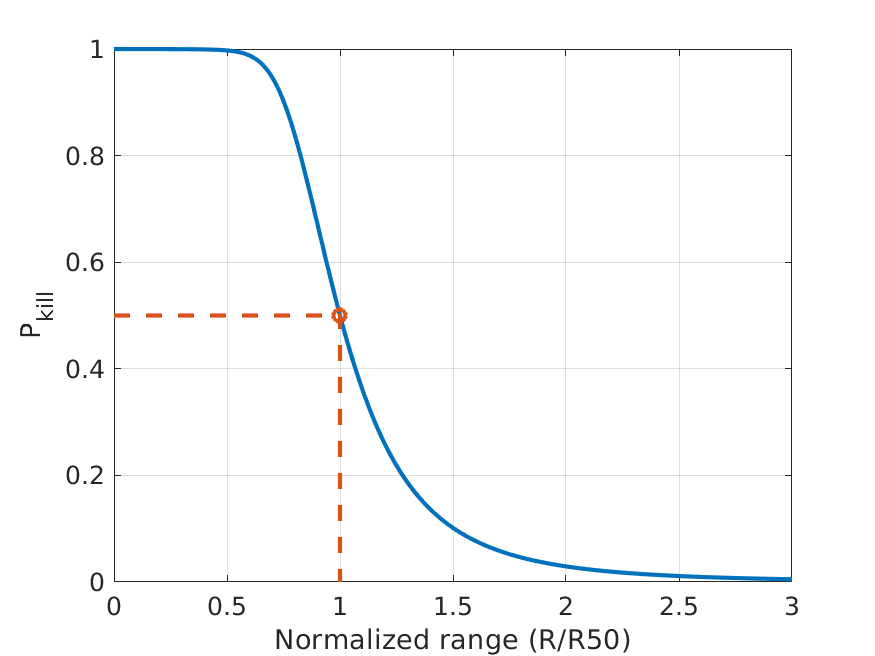
\includegraphics[width=.7\textwidth]{images/pkill.png}
    \caption{$P_k$ as a function of $\frac{R}{R50}$}
    \label{fig:my_label}
\end{figure}

\section{Parameters}

The environment has a lot of parameters that allow to modify its characteristics and working. Those parameters, description and default values are to be found in table \ref{tab:env params}. \\\underline{Note:} One cell $=$ the distance between two adjacent cells.

\begin{table}[h!]
    \centering
    \begin{tabular}{|c|c|c|}
        \hline
        Parameter &  Description &  Default value \\\hline 
        \textit{size} & Size of the grid & $5\times5$ \\\hline 
        \textit{players\_description} & Start position and team of each tank & \makecell{One tank per team\\ Random start position}\\\hline
        \textit{visibility} & Maximum observable range (euclidean distance) & 4 cells \\\hline
        \textit{R50} & Range at which $P_{h}=50\%$ & 3 cells\\\hline
        \textit{obstacles} & List of coordinates of all obstacles in the grid & No obstacles\\\hline
        \textit{borders\_in\_obstacles} & Edges of the grid added to obstacles & False\\\hline
        \textit{max\_cycles} & Maximum number of transitions (-$1=$ no limit) & -$1$ \\\hline
        \textit{max\_ammo} & Maximum number of shots per tank  (-$1=$ no limit) & -$1$ \\\hline
        \textit{im\_size} & Number of pixels in height of the render image & 480\\\hline 
    \end{tabular}
    \caption{Parameters of the \textit{tanksEnv} environment}
    \label{tab:env params} 
\end{table}


\section{Rendering}

Two rendering are possible: A rendering of the full environment, as 

